\documentclass[a4paper]{article}
\usepackage[pdftex]{graphicx}
\usepackage[utf8]{inputenc}
\usepackage{enumerate}
\usepackage{siunitx}
\sisetup{locale=DE}
\usepackage{icomma}
\usepackage{amssymb}
\usepackage{tikz}
\usepackage{href-ul}
\hypersetup{
	colorlinks=true,
	linkcolor=blue,
	urlcolor=blue}
\usepackage{geometry}
\geometry{a4paper, top=15mm, left=15mm, right=15mm, bottom=15mm,
	headsep=10mm, footskip=12mm}

\begin{document}
	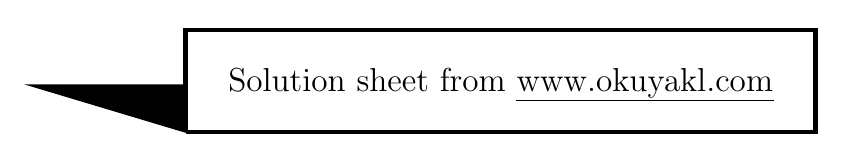
\begin{tikzpicture}(10,3)
		\draw[ultra thick](2,0) --(10,0) -- (10,1.3) --(2,1.3) -- (2,0);
		\draw[fill=black](2,0)-- (0,.6) -- (2,.6) -- (2,0);
		\node at (6,.6) {\large Solution sheet from \href{http://www.okuyakl.com}{www.okuyakl.com}};
	\end{tikzpicture}
	\vspace{0.5 cm}
	
	
	\noindent{\bf Task 1. a)}\\
	These are conductor characteristics
	
	\begin{itemize}
		\item 1: Pencil lead. As the current flow increases, the temperature increases, the conductivity increases and the curve rises.
		\item 2: Iron wire. As the current flow increases, the temperature increases, the conductivity decreases and the curve flattens.
		\item 3: Constantan wire. Conductivity is independent of temperature. The gradient remains constant.
	\end{itemize}
	\vspace{0.5 cm}
	
	\noindent{\bf Task 1. b)}\\
	At $\SI{4}{\volt}$ the iron conductor shows the highest current flow. We read: $I =\SI{1,2}{\ampere}$
	The electrical resistance of this piece of conductor is:
	$$R={U \over I} = {\SI{4,0}{\volt} \over \SI{1,2}{\ampere}}\approx \SI{3,3}{\ohm} $$
	\vspace{0.5 cm}
	
	\noindent{\bf Task 1. c)}\\
	As the voltage increases, the iron wire heats up. In the atomic lattice of iron, the atomic cores now vibrate more strongly and increasingly get in the way of the flowing electrons. The resistance is increasing.
	\vspace{0.5 cm}
	
	\noindent{\bf Task 1. d)}\\
	\begin{itemize}
		\item A PTC thermistor is a PTC, which means positive temperature coefficient. This conducts better at low temperatures.
		\item A thermistor is an NTC, which means negative temperature coefficient.
		This conducts better at high temperatures.
	\end{itemize}
	\vspace{0.5 cm}
	
	\noindent{\bf Task 2. a)}\\
	\renewcommand{\arraystretch}{1.5}
	\begin{tabular}{cccccccc}
		$U$ in V & 0 & 1.8 & 3.6 & 5.4 & 7.2 & 9.0 & 10.8 \\
		\hline
		$I$ in A & 0 & 0.31 & 0.55 & 0.74 & 0.84 & 0.93 & 0.96 \\
		$R$ in $\SI{}{\ohm}$ & - & 5.8 & 6.5 & 7.3 & 8.6 & 9.7 & 11
	\end{tabular}
	
	\noindent
	In conductor 1 you can clearly see the increase in resistance as the current flow increases.
	\vspace{0.5 cm}
	
	\noindent
	\begin{minipage}{0.5\textwidth}
		\noindent{\bf Task 2. b)}\\
		The slope of the graph is the same everywhere. This means that the ratio of voltage to current, the resistance $R$, always remains the same.
		\vspace{0.5 cm}
		
		\noindent{\bf Task 2. c)}\\
		Conductor 1 conducts better when it is cold, while for conductor 2 the temperature does not play a role in the resistance. The resistance of conductor 2 is constant $\SI{10}{\ohm}$.
		\vspace{0.5 cm}
		
		\noindent{\bf Task 3. a)}\\
		The resistance is calculated with:
		$$R={U\over I} = {\SI{6,0}{\volt} \over \SI{5,0}{\ampere}}=\SI{1,2}{\ohm}$$
	\end{minipage}
	\hspace{1cm}
	\begin{minipage}{0.5\textwidth}
		\includegraphics[width=7 cm]{beleik185}
	\end{minipage}
	\vspace{0.5 cm}
	
	\noindent{\bf Task 3. b)}\\
	We apply Ohm's law again and get:
	$$U = R \cdot I = \SI{50}{\ohm} \cdot \SI{0.38}{\ampere} = \SI{19}{\volt}$$
	\vspace{0.5 cm}
	
	\noindent
	
	\noindent{\bf Task 3. c)}\\
	The electrical power is:
	$$P = U \cdot I \quad \Rightarrow \quad I = {P \over U} = {\SI{40}{\watt} \over \SI{230}{\volt}}=\SI{0 ,17}{\ampere}$$
	The resistance is therefore:
	$$R = {U \over I} = {U^2 \over P} = {(\SI{230}{\volt})^2\over \SI{40}{\watt}}=\SI{ 1.3}{\kilo\ohm}$$
	
	\vspace{0.5 cm}
	
	\noindent{\bf Task 3. d)}\\
	Again is:
	$$U = R \cdot I = \SI{1000}{\ohm} \cdot \SI{0.015}{\ampere} = \SI{15}{\volt}$$
	\begin{center}
		\includegraphics[width=7 cm]{../../viecher/eendcomic.pdf}
		
		Here you can go back to the \href{https://www.okuyakl.de/phys/p8widL185/ae185.pdf}{task sheet}
	\end{center}
	
\end{document}